%
% File: chap01.tex

\let\textcircled=\pgftextcircled
\chapter{Stationarity}
\label{chap:stationarity}

\import{}{"chapter_4b_content.tex"}

%\initial{B}egins a chapter. Example: When the beloved cellist (Christopher Walken - outstanding) of a world-renowned string quartet receives a life-changing diagnosis, the group's future suddenly hangs in the balance: suppressed emotions, competing egos and uncontrollable passions threaten to derail years of friendship and collaboration. Featuring a brilliant ensemble cast (including Philip Seymour Hoffman, Catherine Keener and Mark Ivanir as the three other quartet members), it is a fascinating look into the world of working musicians, and an elegant homage to chamber music and the cultural world of New York. The music, of course, is ravishing (the score is the work of regular David Lynch collaborator Angelo Badalamenti): A Late Quartet hits all the right notes.

%
\section{Response of ecological metrics}
\label{sec:results}

%Commented out here. No change from previous version.

For both habitat loss scenarios there is no loss of species richness up to $90 \%$ habitat loss. However significant changes are observed in metrics relating to community composition, network properties and stability. In general the qualitative response of these metrics is not governed by MAI ratio i.e. the direction of the trends are the same across MAI ratios, although the extent of the response may vary.

\begin{figure} 
		\centering      
		\subbottom[What]{
        %\begin{subfigure}[b]{0.5\textwidth}
                \includegraphics[width=0.45\linewidth]{"random_plots/Total abundance"}}
%
        ~
        \subbottom[What]{
        %\begin{subfigure}[b]{0.5\textwidth}
                \includegraphics[width=0.45\linewidth]{"contiguous_plots/Total abundance"}}
        %\end{subfigure}

        \caption{\textbf{Mean total number of individuals} across replicate commmunities decreases with habitat loss, for all MAI ratios. Left: random destruction. Right: contiguous destruction.}\label{fig:total_abundance}
\end{figure}

Although habitat destruction does not lead to extinctions, it does reduce the total biomass of the communities. This is measured by the total number of individuals of all species remaining at the end of a simulation, which we average across replicate communities. Figure \ref{fig:total_abundance} shows that, although mutualistic communities contain more biomass, the loss of biomass due to habitat destruction is ubiquitous. This is not surprising.

\begin{figure} 
		\centering      
        \begin{subfigure}[b]{0.5\textwidth}
                \includegraphics[width=\textwidth]{"random_plots/mean_cv"}
        \end{subfigure}%
        ~
        \begin{subfigure}[b]{0.5\textwidth}
                \includegraphics[width=\textwidth]{"contiguous_plots/mean_cv"}
        \end{subfigure}
        \caption{\textbf{Mean CV in total biomass} across replicate commmunities against habitat loss for selected MAI ratios. Left: random destruction leads to an increase in temporal stability, as indicated by a decrease in CV. Right: contiguous destruction drammatically reduces temporal stability.}\label{fig:temporal_stability}
\end{figure}

How community stability is affected by loss of habitat is of particular interest. Temporal stability is measured by the coefficient of variation (CV) of the total biomass of the system. (This metric is calculated over a number of iterations after the transient dynamics.) A higher CV indicates lower stability, because there are greater fluctuations in the dynamics. We observe that temporal stability is affected differently by the two habitat loss scenarios. As shown in figure \ref{fig:temporal_stability}, random destruction increases temporal stability, whereas contiguous destruction decreases it. What is driving this different response in the dynamics?    

\begin{figure} 
		\centering      
        \begin{subfigure}[b]{0.5\textwidth}
                \includegraphics[width=\textwidth]{"random_plots/IS3"}
        \end{subfigure}%
        ~
        \begin{subfigure}[b]{0.5\textwidth}
                \includegraphics[width=\textwidth]{"contiguous_plots/IS3"}
        \end{subfigure}
        \caption{\textbf{Interaction strengths:} The sum of the elements of the interaction matrix, averaged over replicate commmunities, for selected MAI ratios. Left: random destruction reduces total interaction strength. Right: contiguous destruction drammatically increases total interaction strength.}\label{fig:IS3}
\end{figure}

From figure \ref{fig:IS3} it is clear that the response in temporal stability is closely correlated with interaction strengths, as measured by the metric IS3. Random habitat destruction is characterised by a decrease in total interaction strength, whereas contiguous destruction results in a dramatic increase. It is reasonable to assume that these changes in IS3 are causing the different responses in temporal stability. This is supported by the literature, where it is well documented that strong trophic interactions destabilise population dynamics [REFERENCES]. It is not so obvious what affect on dynamics should be expected from an increase in the strength of mutualistic interactions, which are included in this metric. However, figures \ref{fig:temporal_stability} and \ref{fig:IS3} suggest that this is also destabilising.

\begin{figure} 
		\centering      
        \begin{subfigure}[b]{0.5\textwidth}
                \includegraphics[width=\textwidth]{"random_plots/interaction_strength_distributions"}
                \caption{Random destruction}
        \end{subfigure}%
        ~
        \begin{subfigure}[b]{0.5\textwidth}
                \includegraphics[width=\textwidth]{"contiguous_plots/interaction_strength_distributions"}
                \caption{Contiguous destruction}
        \end{subfigure}
        \caption{\textbf{IS3 distributions:} The interaction strength distribution shifts leftwards for random habitat loss, and rightwards for contiguous loss. The extent of this shift is mediated by MAI ratio - it is most visibile for MAI$=0$, and least visbile for MAI$=1$.}\label{fig:IS3_distributions}
\end{figure}

The trends in total interaction strength are due to underlying shifts in the distribution (figure \ref{fig:IS3_distributions}). This is made visible by a shift in the modal peak to lower or higher interaction strengths, for random or contiguous loss respectively. The extent of this shift is mediated by MAI ratio, with greater shifts for lower levels of mutualism.


\begin{figure}[ht!]
		\centering      
        \includegraphics[width=\textwidth]{"comparison_plots/compare_moransI_mean"}
        \caption{\textbf{Spatial autocorrelation:} Moran's I is calculated for all species distributions and averaged over the community. These plots show the results averaged over all replicates and over all MAI ratios. Solid lines indicate the mean value, and shaded areas indicate $\pm 1$ standard deviation. This metric suggests that species distributions, on average, become less aggregated in space due to random destruction. Whereas they appear to become more spatially aggregated as a result of contiguous destruction.}\label{fig:morans_i}
\end{figure}


What is causing the different responses of IS3 to the different habitat loss scenarios? Spatial aggregation of species distributions is quantified using Moran's I [REFERENCE]. According to this metric, species distributions become less aggregated in space as a result of random destruction (figure \ref{fig:morans_i}). Whereas they appear to become more aggregated in space under contiguous destruction. If species are more aggregated in space, it may be easier to find an interaction partner. This would benefit predators (and mutualists), potentially leading to stronger de-stabilising trophic interactions. The mean frequency of interactions (figure \ref{fig:IS1}) shows some evidence for this effect. On average there are fewer interactions in communities suffering random habitat destruction, than those with contiguous destruction. However the difference is small, suggesting another mechanism is required to explain the strong responses of IS3 and temporal stability. 


It is likely that other changes in network properties and community composition can explain the changes in IS3. The elements of the interaction matrix, used to calculate IS3 are given by \cite{wootton2005measurement, berlow2004interaction}:

\begin{equation}
\alpha_{ij} = \frac{b_{ij}}{N_i N_j},
\end{equation} 

where $\alpha_{ij}$ is the effect of species $j$ on species $i$; $b_{ij}$ is the biomass flow from $i$ to $j$ (here measured by the frequency of the interaction, equivalent to IS1) and $N_i$, $N_j$ are the number of individuals belonging to species $i$ and $j$ respectively. Therefore the elements of the interaction matrix are dependent on the relative abundances of the interacting species, as well as the frequency of the interaction. A more detailed analysis of community composition will let us explain to observed trends.    




%This result seems intuitive since and may explain the different responses in IS3. In the case of contiguous loss individuals are contained within a smaller heterogeneous landscape. This effectively reduces the search space for an interaction partner (although the number of potential interaction partners also decreases).  Whereas random loss effectively introduces barriers to dispersal within a landscape of the same total size. 

 
%\footnote{It should also follow that this effect benefits mutualist species - can we test for this? What does the literature have to say about the effects of stronger mutualistic interactions on temporal stability?}.   

    
\begin{figure} 
		\centering      
        \includegraphics[width=0.6\textwidth]{"comparison_plots/comparing_mean_IS1"}
        \caption{\textbf{Interaction frequencies:} The metric for interaction strength IS1 averaged over all replicates and all MAI values. This metric is the sum of the elements of the interaction frequency matrix i.e. the total number of interaction occuring within a given period of time. Solid lines indicate the mean value, and shaded areas indicate $\pm 1$ standard deviation. For contiguous destruction interactions are slighty more frequent, on average, than for random destruction.}\label{fig:IS1}
\end{figure}

\newpage
\section{More preliminary results}
\label{sec:more_results}

By averaging results over MAI ratios we are able to effectively obtain more replicate communities. When doing this certain metrics appear to display trends in response to habitat loss that are not clearly visible without this averaging. We perhaps need to justify this approach, and to fit statistical models to quantify the significance of the trends in certain metrics. 


\begin{figure}[b!]
		\centering      
        \includegraphics[width=\textwidth]{"comparison_plots/compare_shannoneq_mean"}
        \caption{\textbf{Shannon evenness:} average over MAI ratios and replicate communities. Under random habitat destruction communities on average become more even. Under contiguous destruction there is no change.}\label{fig:shannon_eq}
\end{figure}

\begin{figure}
		\centering      
        \includegraphics[width=\textwidth]{"comparison_plots/compare_h2_mean"}
        \caption{\textbf{Specialisation:} H2' is a metric that qunatifies the degree of specialisation of interactions in the mutualistic sub-network. Mutualists appear to become less specialised under random destruction, and more specialised under contiguous. (This appears to disagree with previous plots of H2, but I can't see why - the numbers used are taken from output\_network.csv, column titled H2.) }\label{fig:h2}
\end{figure}

\begin{figure}[p] 
		\centering      
        \includegraphics[width=\textwidth]{"random_plots/RADs_mut0"}
        \caption{\textbf{RADs for Random habitat loss:} Rank abundance distributions for MAI$=0$, three replicate communities shown for slelected levels of habitat loss (0,50,90). In the case of random destruction we expect the communities to become more even on average, based on Shannon\_Eq metric, (figure \ref{fig:shannon_eq})}\label{fig:RADS_random}
\end{figure}


\begin{figure}[p] 
		\centering      
        \includegraphics[width=\textwidth]{"contiguous_plots/RADS_mut0"}
        \caption{\textbf{RADs for Contiguous habitat loss:} Rank abundance distributions for MAI$=0$, three replicate communities shown for slelected levels of habitat loss (0,50,90). In the case of contiguous destruction we expect no trend in evenness on average, based on Shannon\_Eq metric, (figure \ref{fig:shannon_eq})}\label{fig:RADS_contiguous}
\end{figure}


\section{Further development and work to do}

\subsection{Work to do}

\begin{itemize}
	\item Write introduction
	\item Write up ecological metrics
	\item Amend figure captions
	\item Plot example networks
	\item Plot dynamics
	\item Analyse dynamics (transience, steady-state)
	\item Fix conflict in trophic level results
	\item Analyse ecological metrics by trophic level (basal, intermmediate, top)
	\item Understanding IS3 response: plot $IS1/N^2$, look at individual runs
	\item Compare movement of species to diffusion coefficient in porous medium
	\item Plot RADS with species coloured accroding to trophic level.
\end{itemize}

\subsection{Further development}

\begin{itemize}
	\item Run simulations with lower immigration
	\item Well mixed approximation. Simplified model for analysys
	\item Can we calculate robustness from network, and test this against what extinctions we get? (With lower immigration)
\end{itemize}


%\import{"/home/rusty/Documents/phd files/habitat_loss_project/writings/chapter_2/"}{"chapter_2_content.tex"}
%\import{}{"introduction.tex"}
%\import{}{"chapter_3_content.tex"}
%
%%=======
%\section{Section}
%\label{sec:sec01}
%
%Begins a section.
%
%\subsection{Subsection}
%\label{subsec:subsec01}
%
%Begins a subsection.
%
%%A figures matrix.
%\begin{figure}[t!]
%\centering
%\begin{minipage}{3.3cm}
%    \centering
%    \subtop[]{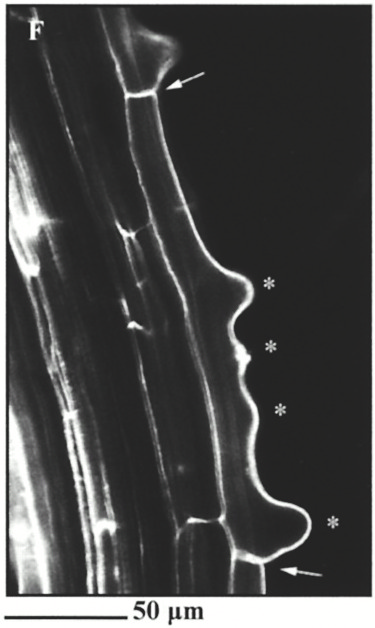
\includegraphics[height=0.28\textheight]{fig01/Nswellings}\label{sf:multiRH02a}}
%\end{minipage}
%\hspace{0.5cm}
%\begin{minipage}{3.3cm}
%    \centering
%    \subtop[]{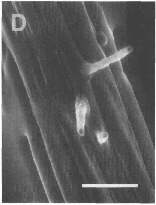
\includegraphics[height=0.27\textheight]{fig01/Mswellings}\label{sf:multiRH02b}}
%\end{minipage}
%\hspace{1.3cm}
%\begin{minipage}{3.3cm}
%    \centering
%    \subtop[]{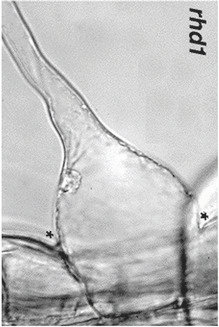
\includegraphics[height=0.27\textheight]{fig01/rhd1}\label{sf:multiRH02c}}
%\end{minipage}
%\\ \vspace{0.1cm}
%\begin{minipage}{10cm}
%    \centering
%    \subtop[]{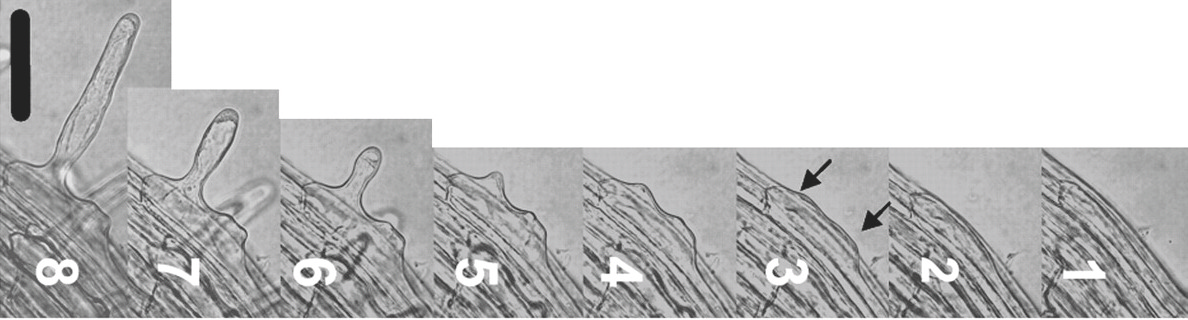
\includegraphics[height=0.145\textheight]{fig01/mutantrhd6}\label{sf:multiRH02d}}
%\end{minipage}
%\\ \vspace{0.1cm}
%\begin{minipage}{10cm}
%    \centering
%    \subtop[]{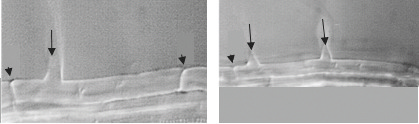
\includegraphics[height=0.16\textheight]{fig01/auxab}\label{sf:multiRH02e}}
%\end{minipage}
%\mycaption[Hair-forming mutant cells.]{(a) A mutant RH cell. Asterisks show multiple sites of RH initiation in a single root hair cell (indicated by the arrows). Figure reproduced from \cite{rigas01}. (b)~Hair-forming cell with three RH initiation locations. The bar represents $50\mu m$. Figure reproduced from \cite{massuci01}. (c) Large bump in mutant {\itshape rhd1}. Figure reproduced from \cite{griersonRH}. (d) Mutant overexpressing gene {\itshape ROP2}; from right-hand to left-hand, numbers indicate progressive snapshots at different times. RH initiation sites are indicated by the arrows. The bar represents $75\mu m$. Figure reproduced from~\cite{mjones01}. (e)~Mutants affected by auxin. On the left-hand side, RH site is farther away from the apical end (left arrow cap); on the right-hand side, multiple RH locations (arrows). Figure reproduced from~\cite{payne01}.}
%\label{fig:multiRH02}
%\end{figure}
%
%% A single figure
%\begin{figure}[t!]
%	\centering
%	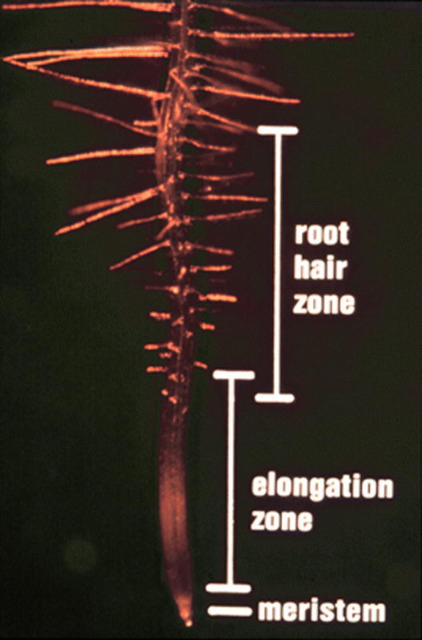
\includegraphics[height=0.35\textheight]{fig01/devepzones}
%	\mycaption[Developmental zones of an Arabidopsis root.]{Developmental zones of an Arabidopsis root. Figure reproduced from \cite{griersonRH}.}
%	\label{fig:RHP02}
%\end{figure}
%
%%=========================================================